

To generate synthetic data and thereby enable sharing of genetic data without privacy concerns we train a diffusion model on real data to produce an arbitrary amount of synthetic data.
\subsection{Data}

Although in this work we establish a model that is generic with respect to the kind of SNPs of a human genome it can predict, we focus on the occurrence/prevalence of ALS as a phenotype in the following. The reasons for this are the availability of the excellent, sufficiently large amounts of data that were raised in the frame of Project MinE \citet{project2018project}. Most importantly, we emphasize ALS, based on the aforementioned large missing heritability. For analogous reasons, also the earlier related studies \citep{auer2012imputation, dolzhenko2017detection} rely on data raised in the frame of Project MinE. 


The data on which we are working on has 18.279 genes sequenced for 10.405 humans. Each of these genes is a sequence of between 5-100 different SNPs.


\subsection{Data Pre-processing}
First we take a closer look at the available data and how it can be compressed to facilitate deep learning on it.% For this compression we closesly follow already established methods \citep{capsulenet}.

A human genome consists of 3 billion base pairs. Analyzing the whole genome for each use case is generally not possible due to its length.
A common alternative in biotech is analyzing the parts of the human genome which change between individual humans. This is done using single nucleotide polymorphisms (SNP). Data in this form is available from \cite{project2018project}.

To further compress this data and make it usable we follow the protocol from \citet{capsulenet}, where these SNPs are individually compressed using Principle Component Analysis (PCA) of varying lengths, up to a maximum of 8 dimensions. This further reduces the dimensionality while incurring minimal compression loss ($<1\%$). A rough outline of this process can be seen in Figure \ref{fig:pca}

\begin{wrapfigure}{r}{0.5\textwidth}
    \centering
    
    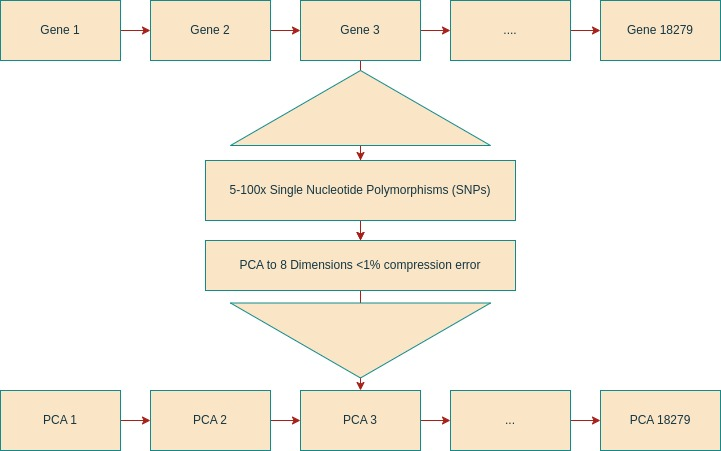
\includegraphics[width = 0.48\textwidth]{figures/preprocess.jpg}
    \caption{Pre-processing pipeline}
    \label{fig:pca}
\end{wrapfigure}

For further pre-processing we zero-pad all PCAs to be of length $8$ to produce a vector of $x \in \mathbb{R}^{18279\times8}$ as a representation of our data. We further pad this with zeroes to be $x \in \mathbb{R}^{18432\times8}$ for efficiency gains on modern architectures ($18432$ is divisible by $2^{11}$). We found that all of this zero-padding, while necessary, results in samples leaving the typically input distribution during the diffusion generation process. To remedy this we set the loss $L(x)$ at all zero padded position to zero, as well as modify the diffusion process by clamping all zero padded positions of $x_p$ to zero. Note that the zero padding is the same for all inputs, so this operation is easy and efficient to apply.


%See Methods for exact descriptions of the data. Note that available data is hard to come by in a real life setting. We focus on data produced by https://www.projectmine.com/ which is high quality whole human genome analysis with a large amount of SNPs analyzed.

\begin{wrapfigure}{r}{0.5\textwidth}
    \centering
    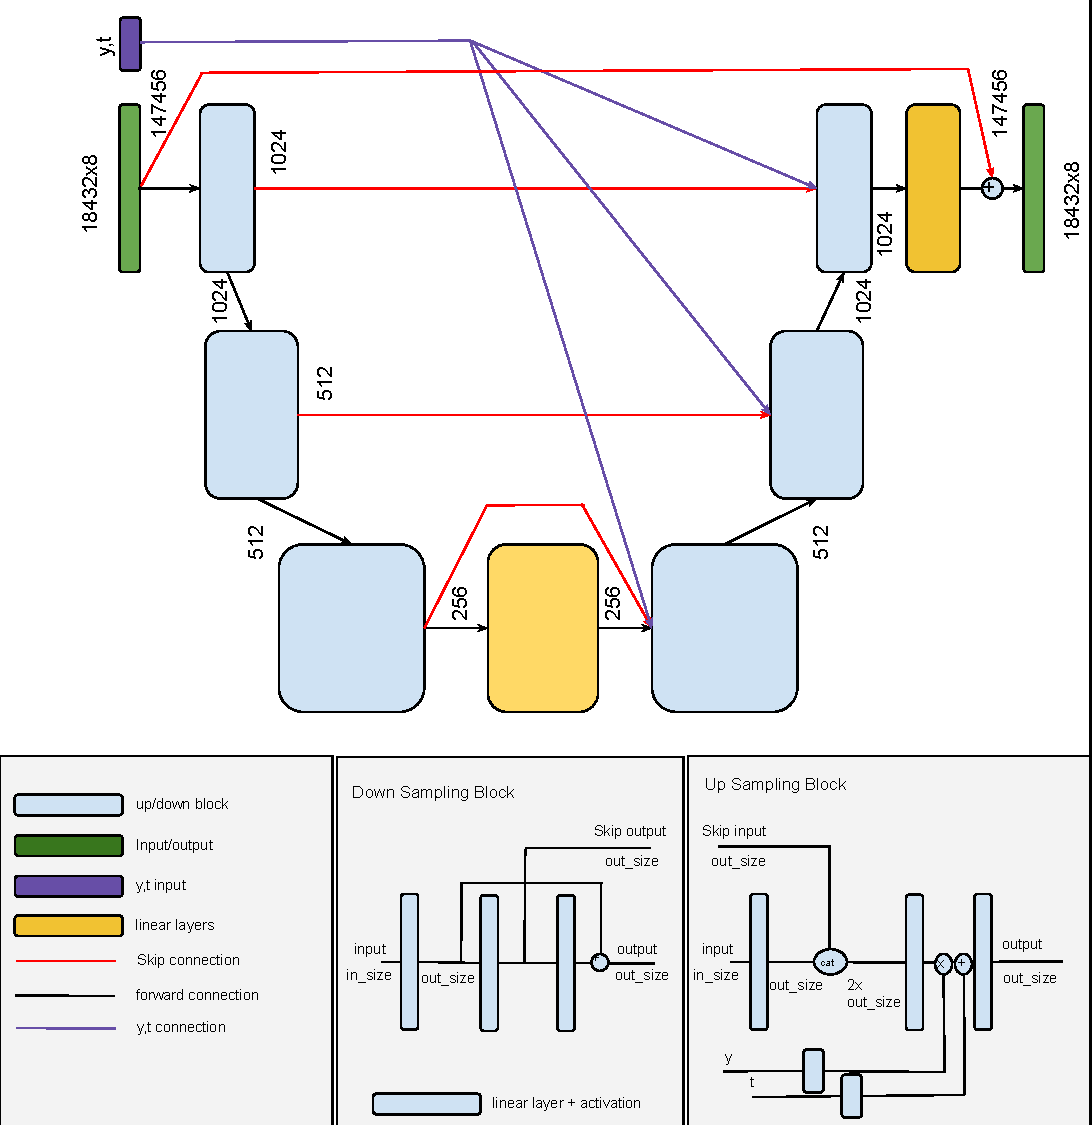
\includegraphics[width = 0.48\textwidth]{figures/UnetMLP.pdf}
   % \includefigure[width = 0.48\textwidth]{figures/UnetMLP.pdf}
    \caption{A structural overview of the architecture of the MLP diffusion model.}
    \label{fig:unet}
\end{wrapfigure}

\subsection{Model Architecture}
We base our Diffusion Model on the popular Unet Architecture by \citet{Unet} but make some changes due to the sequential nature of genetic data.
We evaluate multiple possible Unet architectures where we replace the 2D variants of convolutions with their 1D equivalents or with a Multi-Layer-Perceptron. Another variant which was tried, was a standard transformer encoder structure similar to the one in \cite{bert}, but with learnable positional embeddings, as well as two additional tokens to inject the time $t$ and class $y$ information and an embedding layer similar to the one used for images in VIT\citep{vit} to reduce the number of input tokens. In Figure \ref{fig:unet} we visualize the proposed UnetMLP architecture. The 1D convolutional architecture includes multi-headed attention in the intermediate layers to share global information, this is very similar to what is done for images and needed to reduce the sequential bias introduced by convolutions.
The dense layer architecture does not incorporate this feature.

In general, we want to point out that the approach using 1-d convolutions introduces a sequential bias, which is not biologicaly motivated, but it greatly limits the amount of parameters which have to be learned.

In contrast, the dense model does not incorporate any bias, but it has been shown in many domains that even though in principle fully connected layers can approximate arbitrary functions, they fail to find suitable solutions due to their over-parameterization.

A fully attention based model like the transformer encoder also does not incorporate any spatial bias and should be suitable for this kind of data.






%Encoding the position of the genomes is highly relevant in the case of a CNN based architecture as the position in the sequence is informing the algorithm which SNP is changed and CNNs normally are positional invariant. This can be done by adding a positional encoding to the embedding.% in our case we achieved superior results by adding a custom linear layer to each input which projects the PCA embedding into a shared embedding space, as visualized in Figure \ref{fig:multilinear}, we further refer to it as MultiLinearLayer. The MultiLinearLayer is able to learn the position/gene specific transformation as needed, but contains a comparatively large amount of parameters which could lead to over-fitting.

\subsection{Combining Models}

Since CNN and MLP based models focus on different aspects of the structure of the genome we suggest combining them into a single network thus eliminating both weaknesses. We call this combination CNN + MLP. We combine them by simply adding the predicted noise of each single model $MLP(x)$ and $CNN(x)$ according to:

\begin{equation}
    \textit{MLP + CNN}(x) = (1-\lambda(t)) \cdot MLP(x) + \lambda(t) \cdot CNN(x)
\end{equation}

where $\lambda(t)$ is a learnable function in the range $[0,1]$, realized by a simple multi layer perceptron with 2 layers which has the noise schedule $t$ as input. %In Figure \ref{fig:losscurvesall} we visualize the newly introduced version. While the MLP+CNN model initially outperforms both single versions during longer training it performs about as well as the CNN based diffusion model.

%In Figure \ref{fig:recerror}, we do not observe improved performance compared to the MLP model and thus do not expect an increase in the quality of generated synthetic data.


In summary we propose 5 different Model architectures for the Diffusion Task: Baseline Model, Unet MLP, Unet CNN, Unet MLP + CNN and Transformer.

% \begin{itemize}
%     \item Baseline Model (simple MLP)
%     \item Unet MLP
%     \item Unet CNN
%     \item Unet MLP + CNN
%     \item Transformer
% \end{itemize}

We perform extensive hyper-parameter tuning on all types of models and present the best performing results.
% \begin{figure}
%     \centering
%     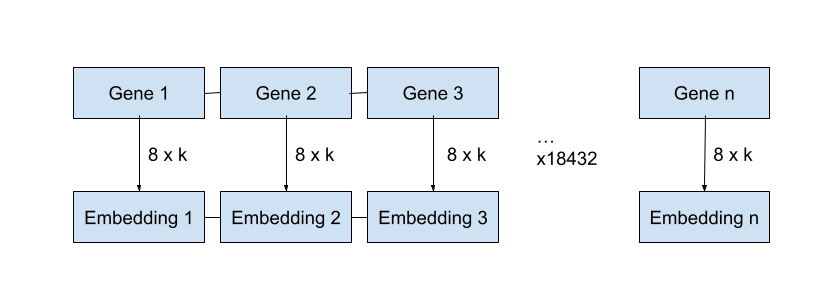
\includegraphics[width = 0.48\textwidth]{figures/MultiLayerLinear.png}
%     \caption{An overview of the proposed MultiLinearLayer}
%     \label{fig:multilinear}
% \end{figure}

\subsection{Evaluation}

The automatic evaluation of genetic diffusion models is a challenging task. Diffusion models were first pioneered in the realm of image generation, where it is comparatively easy to check if the generated data is of high quality. A human is able to inspect the generated images and can manually determine if they are realistic. 
In the genetic case this is no longer possible, as a human observer is not able to easily tell if a genetic sequence is of high fidelity. 


Furthermore, common automatic measurements from the image domain can not be applied to the genetics domain, complicating evaluation. Fréchet inception distance (FID) \citep{fid} and Inception score (IS) \citep{is} are both automatic metrics from the image domain which do not rely on a human observer and are widely regarded as good baselines for synthetic image evaluation. The problem with applying these to the genetic domain is that they rely on models which are pre-trained on large scale data to project images into a meaningful embedding space. While this kind of data is easily available in the image domain, in the genetic domain neither pre-trained models, nor the data to train them, nor data standardization are agreed upon or easy to obtain.

\subsubsection{Nearest Neighbour adversarial accuracy}
To find alternatives to these common scores we look at other scores which compare distributions.
The Nearest Neighbour adversarial accuracy is defined as \cite{yale2019privacy}:

\begin{equation} 
\begin{aligned}
        AA_{truth} = \frac{1}{n}\sum_{i=1}^n \mathbf{1} (d_{TS}(i)>d_{TT}(i)) \\
    AA_{syn} = \frac{1}{n}\sum_{i=1}^n \mathbf{1} (d_{ST}(i)>d_{SS}(i)) \\
   % AA_{TS} = \frac{1}{2}(AA_{truth}+AA_{syn}) \\
  %  PrivacyLoss = Train AA_{TS} - Test AA_{TS}
\end{aligned}
\end{equation}

Where $d(i)$ is denoting the distance of datapoint with index $i$ to the nearest neighbour, $S$ is denoting the synthetic and $T$ the real data origin. For example $d_{ST}(i)$ is the distance between the synthetic datapoint with index $i$ and the nearest neighbour from the real distribution. A score of $AA_{truth} = 0.5$ and $AA_{syn} = 0.5$ is considered optimal. 
% PrivacyLoss denotes the difference between train and test set performance. This should optimally be close to 0.
To calculate the distance to the nearest neighbour $d(i)$ we use the cosine distance metric $d_{cos}$. e.g:

\begin{equation}
    d_{cos}(x,y) = \arccos(\frac{x\cdot y}{|x|\cdot|y|}) \frac{1}{\pi}
\end{equation}

\subsubsection{Nearest Neighbour test}
The nearest neighbour (NN) test with score $S$ compares which distribution the $k$ nearest neighbours belong to.

\begin{equation}
    S(D_1,D_2) = \frac{1}{\#D_1} \sum_{D_1}^x \frac{1}{k}\sum_0^k \delta(x_{k})
\end{equation}

where $\#D$ is the number of samples in $D$ and $x_{k}$ the $k$-th nearest neighbour to $x$ in distribution $D_a = D_1 \cup D_2$, according to some distance metric, we choose the cosine distance metric. We define $\delta(x_k) = 1$ if $x_{k}\in D_1$ and 0 otherwise. An optimal score would be $S = 0.5$.

\subsubsection{UMAP}
Another common evaluation possibility is the visualization of neighbourhood structure using algorithms like UMAP \citep{UMAP} or T-SNE \citep{tsne}. Both of these methods are highly popular in the realm of Machine Learning. We choose to use UMAP due to its better performance on high dimensional data.

% \subsubsection{Linkage disequilibrium}
% Another metric which is specific to the genetic use case is Linkage disequilibrium. This metric correlates the association of alleles of different loci. By comparing the Linkage disequilibrium of our synthetic data to real data we can validate a realistic synthetic data generation.

\subsubsection{Amyotrophic Lateral Sclerosis (ALS) classification}
As the final and most important evaluation metric we use a real life binary classification task. The classification task we choose is to determine whether or not the genetic disease Amyotrophic Lateral Sclerosis is present. This task is especially suitable to evaluate if a realistic genome is produced due to its relatively high complexity, as well as the comparatively large amount of training samples which are present for this task. The task is based on 10.405 examples which were diagnosed by medical professionals into 3192 ALS positive and 7213 negative samples. The task does not exhibit simple reliance on one or even multiple genomes and at least 1000 genomes are needed to obtain good performance \citep{capsulenet}.  

We train a simple classifiers to perform binary classification. If the classifier can also be trained on synthetic data and still performs well on a holdout test set of real data we can conclude that the features used for ALS classification were well reproduced.
To ablate against the type of classifier having a large impact we evaluate using 3 different classifiers: MLP, Transformer and CNN.
% \begin{itemize}
%     \item MLP
%     \item Transformer
%     \item CNN
% \end{itemize}

All evaluations will be performed on a balanced hold out test set of 520 positive and 520 negative examples for a total of 1040 samples or 10\% of the total available data. We follow the experimental protocol of \citet{capsulenet} to achieve easy to compare results.